\documentclass[12pt]{article}
\usepackage[utf8]{inputenc}

\usepackage{report_template}
\usepackage{color}
\usepackage{vwcol} 
\usepackage[
labelfont=sf,
hypcap=false,
calcwidth=1.0\linewidth
]{caption}

\usepackage{Sweave}
\begin{document}
\Sconcordance{concordance:report.tex:report.Rnw:%
1 12 1 1 0 37 1 1 24 11 1 1 55 49 1 1 28 33 1 1 14 26 1 1 5 27 0 1 2 3 %
1 1 12 14 1}


\thispagestyle{firststyle}

{\Large \noindent\textbf{Predicting points in the NHL}}

\medskip
\noindent \textsl{by Nathan Esau, Fernando Villasenor and Steve Kane} \hfill {\footnotesize\url{http://github.com/stat350/nhlmodel}}

\section{Introduction and Motivation}

The point system of the NHL currently awards two points to the winner, one point to a team that loses either in overtime or in a shoot-out, and zero points to a team that loses in regulation time. Our analysis is an attempt to explain the number of points that a team will get in a season using linear regression. The variables in our model include how many goals a team has scored or allowed, how many shots they have taken or allowed, how old their players are, and perhaps other variables. It is important to note that we do not need to know the outcome of any particular game to do this and we are using aggregate quantities to determine a teams current season standing.

Our data is from the 2007--2008 season to the 2014--2015 season -- before this some of our advanced metrics weren't available. A peculiarity of our is that the season of 2012--2013 was affected by a lockout which led to only 48 out of 82 games played (GP). Despite this apparent mixing of data we still use all of the data in our analysis and deal with this problem by scaling certain covariates by the proportion of the season which a team has played.

\section{Exploratory analysis}

Many of the variables in hockey data are redundant. For instance, points summarizes the number of wins, losses and overtime or shootout losses a team has and faceoff percentage summarizes the number of faceoffs a team has won and lost. We tried to choose variables that conveyed different information to avoid colinearity. These variables are shown below.

\begin{table}[ht]
\small
\def\arraystretch{1.2}
\centering
\begin{tabular}{p{1.2cm} p{2.2cm} p{3.5cm} |p{1.2cm} p{2.5cm} p{3.8cm}}
\hline
 & Variable & Description & & Variable & Description\\ \hline
AvAge & Average Age & Age weighted by time on ice & PTS & Points & A measure of a teams success \\ \hline
BLK & Blocks & Blocked shots & S & Shots & Shots on goal \\ \hline
FF\% & Fenwick for percentage & A measure of puck possession & SA & Shots Against & Shots allowed on goal \\ \hline 
GA & Goals Against & Goals allowed & SH & Short-handed goals & Goals scored while on penalty kill \\ \hline
GF & Goals For & Goals scored & SHA & Short-handed goals allowed & Goals allowed while on power play \\ \hline
PK\% & Penalty kill perrcentage & Percentage other team scores on power play & SOS & Strength of schedule & Looks at whether team is good due to weak opponents \\ \hline
PP\% & Power play percentage & Percentage team scores on power play & SRS & Simple rating system & Takes into account average goal differential \\ \hline
\end{tabular} 
\caption{Important hockey statistics used in our analysis}
\end{table}


\begin{vwcol}[widths={0.68,0.32}, sep=0cm, justify=flush, 
rule=0pt, indent=0em] 
%
\begin{minipage}{0.68\linewidth}
\vspace{-15mm}
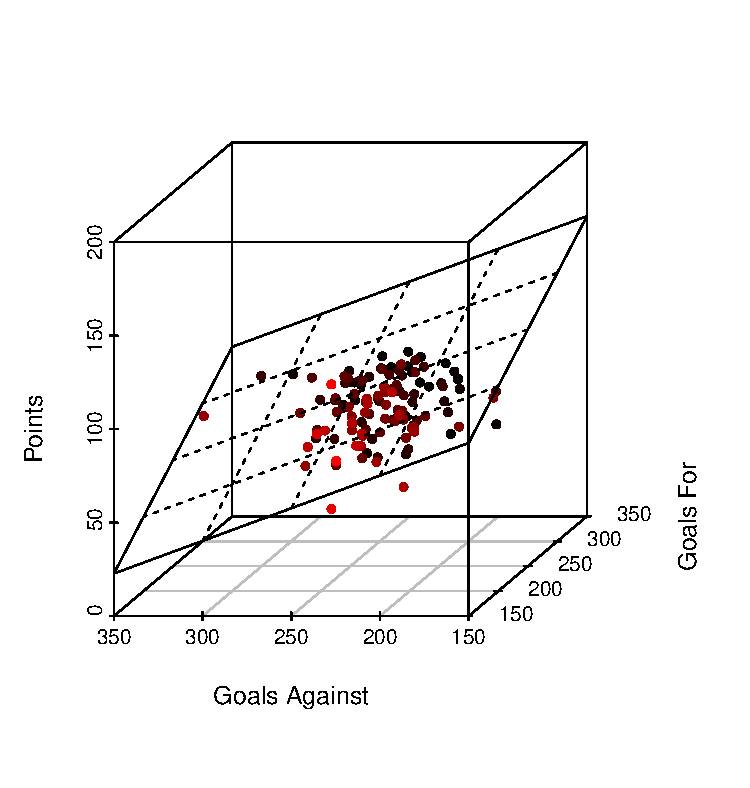
\includegraphics[width=1.0\textwidth]{report-basic_model}
\vspace{-12mm}
\setcounter{figure}{0}
\captionof{figure}{The model PTS = $\beta_{0}$ + $\beta_{1}$ GF + $\beta_{2}$ GA}
\end{minipage}

%
\begin{minipage}{0.32\linewidth}
%\vspace{-10mm}
{\small
\begin{tabular}{l r r }
\hline
\textsl{82 GP} & Mean & SD \\ \hline
\text{AvAge} & 27.84 & 1.16 \\
\text{BLK} & 1119.59 & 151.79 \\
%\text{FF\%} & 50 & 2.82 \\
\text{GF, GA} & 228.88 & 23.5  \\ 
%\textsl{SOS} & 0 & 0.06 \\
%\textsl{SRS} & 0 & 0.43 \\
\text{PK\%} & 81.86 & 2.87 \\
\text{PTS} & 91.83 & 13.26 \\
\text{S, SA} & 2456.1 & 94.89 \\ 
\text{SH, SHA} & 6.75 & 3.1 
\end{tabular} 

\medskip\smallskip
\begin{tabular}{l r r }
\hline
\textsl{48 GP} & Mean & SD \\ \hline
\text{AvAge} & 27.64 & 1.08 \\
\text{BLK} & 686.57 & 83.63 \\
%\text{FF\%} & 50 & 2.82 \\
\text{GF, GA} & 50.04 & 3.09  \\ 
%\textsl{SOS} & 0 & 0.06 \\
%\textsl{SRS} & 0 & 0.43 \\
\text{PK\%} & 81.75 & 3.43 \\
\text{PTS} & 53.4 & 9.64 \\
\text{S, SA} & 1398.8 & 94.89 \\ 
\text{SH, SHA} & 3.1 & 2.26 \\
\end{tabular}}
\setcounter{table}{1}
\captionof{table}{Summary statistics from 2008--2015 for 82 game and 48 game seasons.}
\end{minipage}
\end{vwcol}

\vspace{-25mm}\noindent
A well-known model for predicting points in hockey is PTS = $\beta_{0} + \beta_{1}$ GF + $\beta_{2}$ GA, shown above in Figure 1 for non-lockout seasons. Notice that the dots are nicely scattered around the plane, but there are a few outliers. Later on, we show that it is possible to obtain a model with a lower $R^{2}_{Adj}$ and out of sample MSE by incorporating other variables into the model.

Not all of the variables increase as the number of games played increases. In particular, AvAge, FF\%, PK\%, PP\%, SOS and SRS are relatively stable as the number of games played changes. This is evident by comparing the value of PK\% in the 48 game season to the value of PK\% in the 82 game season in Table 2. Later on in our analysis, when we predict points in the 2015--2016 season, we scale the coefficients of these variables by the proportion of the season which a team has played and obtain the MSE of these predictions.

\section{Methods}

To explain the number of points a team, we used multivariate regression. We used the R function from the \texttt{leaps} package to determine the best model given a certain number of covariates. This function tried all possible combinations of the variables shown in Table 1 given a fixed model size and returned the variables which were most significant (had the smallest $p$-values). We then compared models of different sizes using $R^{2}_{Adj}$ and out of sample MSE (MSPE) based our current season points predictions as at November 21, 2015.

As explained previously, some variables are not proportional to the number of games a team plays. For this reason, some variables such as SRS and SOS did not work very well when including the lockout season in the training set. We fit separate models on two training sets, one of which included the 48 game lockout season and one of which excluded the 48 game lockout season. The models shown in Table 3 and Table 4 use the variables suggested by the \texttt{regsubsets} function.


\begin{table}[ht]
\footnotesize
\def\arraystretch{1.2}
\centering
\begin{tabular}{l |p{1.5cm} |r}
\hline
\textsl{Model} & $R^{2}_{Adj}$ & \textsl{MSPE} \\ \hline
\begin{tabular}{l r r r}
& $\beta_{0}$ & GF & GA \\
coef & 17.86 & 0.51 & -0.2 \\
$p$ & 0 & 0 & 0  \\ 
\end{tabular} & 0.8516 & 9.85 \\ \hline
\begin{tabular}{l r r r r r}
& $\beta_{0}$ & GF & GA & S & SA \\
coef & 8.57 & 0.35 & -0.32 & 0.02 & 0.01 \\
$p$ & 2e-04 & 0 & 0 & 0 & 0  \\ 
\end{tabular} & 0.9093 & 5.1538 \\ \hline
\begin{tabular}{l r r r r r r r}
& $\beta_{0}$ & AvAge & GF & GA & SRS & S & SA \\
coef & -15.58 & 0.86 & 0.21 & -0.17 & 11.43 & 0.02 & 0.01 \\
$p$ & 0.0749 & 0.0051 & 0 & 8e-04 & 0.004 &  0 &  0  \\ 
\end{tabular} & 0.9144 & 5.3148 \\ \hline
\begin{tabular}{l r r r r r r r r r}
& $\beta_{0}$ & AvAge & GF & GA & SA & FF\% & BLK & SOS & PK\% \\
coef & -116.11 & 0.94 & 0.37 & -0.3 & 0.02 & 1.39 & 0.01 & 18.89 & 0.33 \\
$p$ & 0 & 0.0028 & 0 & 0 & 0 &  0 &  0.0041 &  0.0017 &  0.0189 \\ 
\end{tabular} & 0.9179 & 5.8291 \\ \hline
\end{tabular}
\caption{Models fit to data with 2012--2013 lockout season included}
\end{table}

\medskip\noindent When models were fit to the first training set, we can see that goals for and goals against are important variables followed by shots and shots against. Most of the coefficients have an intuitive explanation. For instance, if a team scores many goals they have a better chance of winning games and getting more points so the coefficient for goals for is positive. There are notable interesting coefficients such as the coefficient for average age, which is positive. This would imply that teams with older players tend to do better than teams with younger players since they have more experience.


\begin{table}[ht]
\footnotesize
\def\arraystretch{1.2}
\centering
\begin{tabular}{l |p{1.5cm} |r}
\hline
\textsl{Model} & $R^{2}_{Adj}$ & \textsl{MSPE} \\ \hline
\begin{tabular}{l r r r r}
& $\beta_{0}$ & SRS & SOS & SH \\ 
coef & 93.83 & 28.66 & -25.7 & -0.29 \\
$p$ & 0 & 0 & 0 & 0.0023  \\ 
\end{tabular} & 0.8992 & 5.3777 \\ \hline
\begin{tabular}{l r r r r r r}
& $\beta_{0}$ & GF & GA & AvAge & SH & SHA \\
coef & 80.5 & 0.34 & -0.35 & 0.49  & -0.27 & 0.2 \\
$p$ & 0 & 0 & 0 & 0.0572 & 0.0052 & 0.0486   \\ 
\end{tabular} & 0.9119 & 5.2594 \\ \hline
\end{tabular}
\caption{Models fit to data with 2012--2013 lockout season excluded}
\end{table}

\medskip\noindent For the second training set, we can see that goals for and goals against are no longer the most significant variables in small models, replaced instead by the simple rating system and strength of schedule metrics. When models were fit to this training set we found that $R^{2}_{Adj}$ values were smaller, most likely as a result of using less data when fitting the model. We ended up choosing the model PTS = $\beta_{0}$ + $\beta_{1}$GF + $\beta_{2}$GA + $\beta_{3}$S + $\beta_{4}$SA since it had the best MSPE, comparable $R^{2}_{Adj}$ to other models and is a model which is easy to interpret. 

\section{Results}

\vspace{-5mm}
% latex table generated in R 3.2.2 by xtable 1.8-0 package
% Sun Nov 22 18:11:16 2015
\begin{table}[ht]
\centering
{\small
\begin{tabular}{lrr|lrr}
  \hline
Team & Actual & Predicted & Team & Actual & Predicted \\ 
  \hline
Anaheim Ducks & 18 & 17.62 & Montreal Canadiens & 32 & 32.75 \\ 
  Arizona Coyotes & 21 & 19.70 & Nashville Predators & 25 & 22.70 \\ 
  Boston Bruins & 19 & 21.61 & New Jersey Devils & 21 & 18.23 \\ 
  Buffalo Sabres & 18 & 17.92 & New York Islanders & 23 & 24.99 \\ 
  Calgary Flames & 17 & 15.01 & New York Rangers & 30 & 28.66 \\ 
  Carolina Hurricanes & 15 & 13.91 & Ottawa Senators & 23 & 21.83 \\ 
  Chicago Blackhawks & 24 & 23.92 & Philadelphia Flyers & 17 & 15.30 \\ 
  Colorado Avalanche & 15 & 20.82 & Pittsburgh Penguins & 24 & 21.12 \\ 
  Columbus Blue Jackets & 16 & 18.34 & San Jose Sharks & 22 & 21.60 \\ 
  Dallas Stars & 32 & 30.06 & St. Louis Blues & 27 & 23.52 \\ 
  Detroit Red Wings & 22 & 19.49 & Tampa Bay Lightning & 21 & 21.71 \\ 
  Edmonton Oilers & 15 & 19.01 & Toronto Maple Leafs & 18 & 19.91 \\ 
  Florida Panthers & 19 & 21.45 & Vancouver Canucks & 20 & 22.90 \\ 
  Los Angeles Kings & 24 & 23.14 & Washington Capitals & 25 & 23.50 \\ 
  Minnesota Wild & 23 & 19.91 & Winnipeg Jets & 20 & 19.66 \\ 
   \hline
\end{tabular}
}
\caption{Predictions for 2015--2016 season at November 21, 2015 using the model PTS = $\beta_{0}$ + $\beta_{1}$GF + $\beta_{2}$GA + $\beta_{3}$S + $\beta_{4}$SA fit with the lockout season included} 
\end{table}
\noindent
The largest residuals in Table 5 come from the predictions for the Colorado Avalanche and Edmonton Oilers, which both have 15 points. Unlike Carolina, these teams have a near zero goal differential and lost several close games which our model cannot account for. Residual plots for the fitted model and predicted points are shown in Figure 2.


\begin{figure}[!ht]
\begin{center}
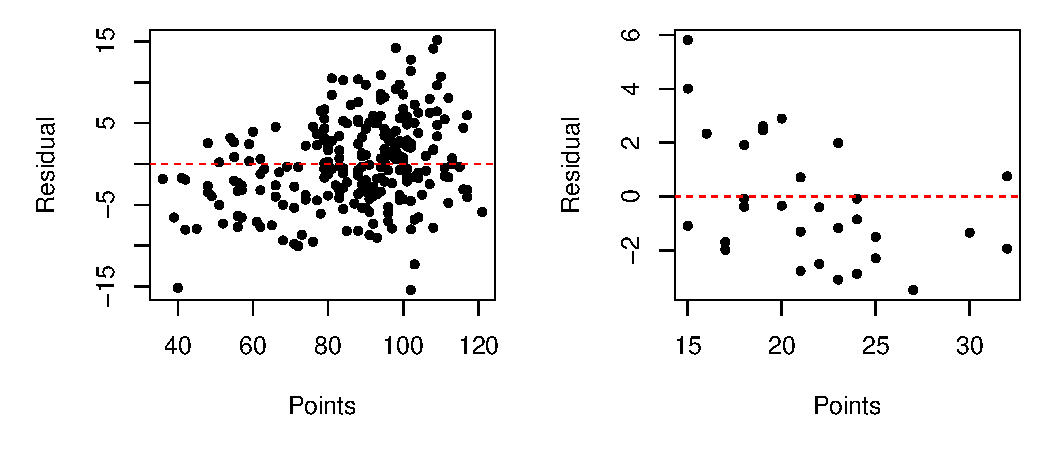
\includegraphics[width=0.9\textwidth]{report-residual_plots}
\end{center}
\vspace{-9mm}
\caption{{\small Residuals (fitted: left; predicted: right) for PTS = $\beta_{0} + \beta_{1}$GF + $\beta_{2}$GA + $\beta_{3}$S + $\beta_{4}$SA}}
\end{figure}

\vspace{-7mm}
\section{Conclusion}

We compared models using $R^{2}_{Adj}$ and MSPE and chose the model PTS = $\beta_{0} + \beta_{1}$GF + $\beta_{2}$GA + $\beta_{3}$S + $\beta_{4}$SA. Our model can estimate the points a team has any time during the season if these variables are known. An area for future work would be to project a teams end of season points, perhaps with the use of a time series model.

\end{document}
